\documentclass[11pt]{amsart}
\usepackage[a4paper,margin=1in]{geometry}
\usepackage{amssymb,amsmath}
\usepackage{tikz}
\usepackage[font=small,labelfont=bf]{caption}
\usepackage[hidelinks]{hyperref}

\colorlet{copper}{orange!75!black}
\colorlet{inkmuted}{black!60}

\newtheorem{theorem}{Theorem}
\newtheorem{lemma}[theorem]{Lemma}
\theoremstyle{remark}
\newtheorem{remark}[theorem]{Remark}

\title{Zeta Along a Semicircle}
\author{Vamshi Jandhyala}
\address{London, United Kingdom}
\email{vamshi.jandhyala@gmail.com}

\begin{document}

\begin{abstract}
A question on Mathematics Stack Exchange asks whether $|\zeta(z)|$ increases strictly along the semicircle $z=1-5e^{iu}$, $0\le u\le\pi$, which runs from the trivial zero $-4$ through the critical strip to $6$. We prove that it does, with a computer-assisted argument in ball arithmetic, and that the same holds for the semicircle of radius $3$ through $-2$. For the semicircles of radius $7,9,\dots,41$ through the other trivial zeros it fails: $|\zeta|$ decreases on a certified interval. A heuristic from the functional equation explains the threshold: once the arc reaches height $2\pi$ while moving to the right in the half-plane $\operatorname{Re}z<0$, $|\zeta|$ falls. The exact reductions behind the computation are checked in Lean.
\end{abstract}

\maketitle

\section{The question}

Start at the trivial zero $z=-4$ of the Riemann zeta function and walk to $z=6$ along the lower semicircle centred at $1$, $z(u)=1-5e^{iu}$ for $0\le u\le\pi$. A Mathematics Stack Exchange user asked whether $|\zeta(z(u))|$ increases strictly along the way, and whether a computer-assisted proof would count~\cite{MSE}. The walk starts at $|\zeta|=0$ and ends at $\zeta(6)=\pi^6/945\approx1.017$, but in between it crosses the critical strip, where $|\zeta|$ can do anything. Before reading on, it is worth guessing what happens on the larger semicircles through $-6$, $-8$, \dots: Figure~\ref{fig:arcs} gives the answer away.

\begin{theorem}\label{thm:main}
For $r=3$ and $r=5$, the function $u\mapsto|\zeta(1-re^{iu})|$ is strictly increasing on $[0,\pi]$.
\end{theorem}

\begin{theorem}\label{thm:fail}
For every odd $r$ with $7\le r\le41$, the function $u\mapsto|\zeta(1-re^{iu})|$ is not monotone on $[0,\pi]$.
\end{theorem}

\begin{figure}[ht]
\centering
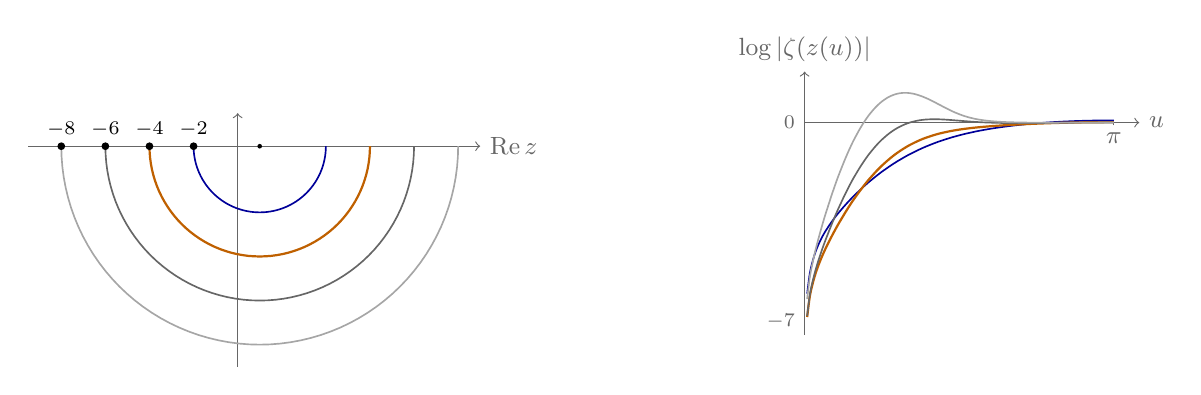
\begin{tikzpicture}[font=\small]
\begin{scope}[scale=0.28]
\draw[inkmuted,->] (-9.5,0) -- (11,0) node[right] {$\operatorname{Re} z$};
\draw[inkmuted,->] (0,-10) -- (0,1.5);
\draw[blue!60!black,semithick] plot coordinates {(-2.000,0.000) (-1.996,-0.157) (-1.984,-0.314) (-1.963,-0.469) (-1.934,-0.624) (-1.898,-0.776) (-1.853,-0.927) (-1.801,-1.075) (-1.741,-1.220) (-1.673,-1.362) (-1.598,-1.500) (-1.516,-1.634) (-1.427,-1.763) (-1.331,-1.888) (-1.229,-2.007) (-1.121,-2.121) (-1.007,-2.229) (-0.888,-2.331) (-0.763,-2.427) (-0.634,-2.516) (-0.500,-2.598) (-0.362,-2.673) (-0.220,-2.741) (-0.075,-2.801) (0.073,-2.853) (0.224,-2.898) (0.376,-2.934) (0.531,-2.963) (0.686,-2.984) (0.843,-2.996) (1.000,-3.000) (1.157,-2.996) (1.314,-2.984) (1.469,-2.963) (1.624,-2.934) (1.776,-2.898) (1.927,-2.853) (2.075,-2.801) (2.220,-2.741) (2.362,-2.673) (2.500,-2.598) (2.634,-2.516) (2.763,-2.427) (2.888,-2.331) (3.007,-2.229) (3.121,-2.121) (3.229,-2.007) (3.331,-1.888) (3.427,-1.763) (3.516,-1.634) (3.598,-1.500) (3.673,-1.362) (3.741,-1.220) (3.801,-1.075) (3.853,-0.927) (3.898,-0.776) (3.934,-0.624) (3.963,-0.469) (3.984,-0.314) (3.996,-0.157) (4.000,-0.000)};
\node[blue!60!black,below,font=\scriptsize] at (-2,-0.2) {};
\draw[copper,thick] plot coordinates {(-4.000,0.000) (-3.993,-0.262) (-3.973,-0.523) (-3.938,-0.782) (-3.891,-1.040) (-3.830,-1.294) (-3.755,-1.545) (-3.668,-1.792) (-3.568,-2.034) (-3.455,-2.270) (-3.330,-2.500) (-3.193,-2.723) (-3.045,-2.939) (-2.886,-3.147) (-2.716,-3.346) (-2.536,-3.536) (-2.346,-3.716) (-2.147,-3.886) (-1.939,-4.045) (-1.723,-4.193) (-1.500,-4.330) (-1.270,-4.455) (-1.034,-4.568) (-0.792,-4.668) (-0.545,-4.755) (-0.294,-4.830) (-0.040,-4.891) (0.218,-4.938) (0.477,-4.973) (0.738,-4.993) (1.000,-5.000) (1.262,-4.993) (1.523,-4.973) (1.782,-4.938) (2.040,-4.891) (2.294,-4.830) (2.545,-4.755) (2.792,-4.668) (3.034,-4.568) (3.270,-4.455) (3.500,-4.330) (3.723,-4.193) (3.939,-4.045) (4.147,-3.886) (4.346,-3.716) (4.536,-3.536) (4.716,-3.346) (4.886,-3.147) (5.045,-2.939) (5.193,-2.723) (5.330,-2.500) (5.455,-2.270) (5.568,-2.034) (5.668,-1.792) (5.755,-1.545) (5.830,-1.294) (5.891,-1.040) (5.938,-0.782) (5.973,-0.523) (5.993,-0.262) (6.000,-0.000)};
\node[copper,below,font=\scriptsize] at (-4,-0.2) {};
\draw[inkmuted,semithick] plot coordinates {(-6.000,0.000) (-5.990,-0.366) (-5.962,-0.732) (-5.914,-1.095) (-5.847,-1.455) (-5.761,-1.812) (-5.657,-2.163) (-5.535,-2.509) (-5.395,-2.847) (-5.237,-3.178) (-5.062,-3.500) (-4.871,-3.812) (-4.663,-4.114) (-4.440,-4.405) (-4.202,-4.684) (-3.950,-4.950) (-3.684,-5.202) (-3.405,-5.440) (-3.114,-5.663) (-2.812,-5.871) (-2.500,-6.062) (-2.178,-6.237) (-1.847,-6.395) (-1.509,-6.535) (-1.163,-6.657) (-0.812,-6.761) (-0.455,-6.847) (-0.095,-6.914) (0.268,-6.962) (0.634,-6.990) (1.000,-7.000) (1.366,-6.990) (1.732,-6.962) (2.095,-6.914) (2.455,-6.847) (2.812,-6.761) (3.163,-6.657) (3.509,-6.535) (3.847,-6.395) (4.178,-6.237) (4.500,-6.062) (4.812,-5.871) (5.114,-5.663) (5.405,-5.440) (5.684,-5.202) (5.950,-4.950) (6.202,-4.684) (6.440,-4.405) (6.663,-4.114) (6.871,-3.812) (7.062,-3.500) (7.237,-3.178) (7.395,-2.847) (7.535,-2.509) (7.657,-2.163) (7.761,-1.812) (7.847,-1.455) (7.914,-1.095) (7.962,-0.732) (7.990,-0.366) (8.000,-0.000)};
\node[inkmuted,below,font=\scriptsize] at (-6,-0.2) {};
\draw[black!35,semithick] plot coordinates {(-8.000,0.000) (-7.988,-0.471) (-7.951,-0.941) (-7.889,-1.408) (-7.803,-1.871) (-7.693,-2.329) (-7.560,-2.781) (-7.402,-3.225) (-7.222,-3.661) (-7.019,-4.086) (-6.794,-4.500) (-6.548,-4.902) (-6.281,-5.290) (-5.994,-5.664) (-5.688,-6.022) (-5.364,-6.364) (-5.022,-6.688) (-4.664,-6.994) (-4.290,-7.281) (-3.902,-7.548) (-3.500,-7.794) (-3.086,-8.019) (-2.661,-8.222) (-2.225,-8.402) (-1.781,-8.560) (-1.329,-8.693) (-0.871,-8.803) (-0.408,-8.889) (0.059,-8.951) (0.529,-8.988) (1.000,-9.000) (1.471,-8.988) (1.941,-8.951) (2.408,-8.889) (2.871,-8.803) (3.329,-8.693) (3.781,-8.560) (4.225,-8.402) (4.661,-8.222) (5.086,-8.019) (5.500,-7.794) (5.902,-7.548) (6.290,-7.281) (6.664,-6.994) (7.022,-6.688) (7.364,-6.364) (7.688,-6.022) (7.994,-5.664) (8.281,-5.290) (8.548,-4.902) (8.794,-4.500) (9.019,-4.086) (9.222,-3.661) (9.402,-3.225) (9.560,-2.781) (9.693,-2.329) (9.803,-1.871) (9.889,-1.408) (9.951,-0.941) (9.988,-0.471) (10.000,-0.000)};
\node[black!35,below,font=\scriptsize] at (-8,-0.2) {};
\fill (-2,0) circle (5pt) node[above,font=\scriptsize] {$-2$};
\fill (-4,0) circle (5pt) node[above,font=\scriptsize] {$-4$};
\fill (-6,0) circle (5pt) node[above,font=\scriptsize] {$-6$};
\fill (-8,0) circle (5pt) node[above,font=\scriptsize] {$-8$};
\fill (1,0) circle (3pt);
\end{scope}
\begin{scope}[xshift=7.2cm,yshift=0.3cm,x=1.25cm,y=0.36cm]
\draw[inkmuted,->] (0,0) -- (3.4,0) node[right] {$u$};
\node[left,inkmuted,font=\scriptsize] at (0,0) {$0$};
\node[left,inkmuted,font=\scriptsize] at (0,-7) {$-7$};
\draw[inkmuted,->] (0,-7.5) -- (0,1.8) node[above] {$\log|\zeta(z(u))|$};
\node[below,inkmuted] at (3.1416,0) {$\pi$};
\draw[inkmuted] (3.1416,-0.1) -- (3.1416,0.1);
\draw[blue!60!black,semithick] plot[smooth] coordinates {(0.026,-6.034) (0.052,-5.335) (0.079,-4.921) (0.105,-4.620) (0.131,-4.381) (0.157,-4.179) (0.183,-4.003) (0.209,-3.845) (0.236,-3.700) (0.262,-3.565) (0.288,-3.438) (0.314,-3.318) (0.340,-3.203) (0.367,-3.093) (0.393,-2.987) (0.419,-2.885) (0.445,-2.787) (0.471,-2.691) (0.497,-2.598) (0.524,-2.508) (0.550,-2.420) (0.576,-2.335) (0.602,-2.252) (0.628,-2.172) (0.654,-2.093) (0.681,-2.017) (0.707,-1.943) (0.733,-1.871) (0.759,-1.801) (0.785,-1.733) (0.812,-1.667) (0.838,-1.603) (0.864,-1.541) (0.890,-1.480) (0.916,-1.422) (0.942,-1.365) (0.969,-1.310) (0.995,-1.257) (1.021,-1.205) (1.047,-1.155) (1.073,-1.107) (1.100,-1.060) (1.126,-1.015) (1.152,-0.971) (1.178,-0.929) (1.204,-0.888) (1.230,-0.849) (1.257,-0.811) (1.283,-0.775) (1.309,-0.739) (1.335,-0.705) (1.361,-0.672) (1.388,-0.641) (1.414,-0.610) (1.440,-0.581) (1.466,-0.553) (1.492,-0.525) (1.518,-0.499) (1.545,-0.474) (1.571,-0.449) (1.597,-0.426) (1.623,-0.403) (1.649,-0.382) (1.676,-0.361) (1.702,-0.341) (1.728,-0.321) (1.754,-0.303) (1.780,-0.285) (1.806,-0.268) (1.833,-0.251) (1.859,-0.235) (1.885,-0.220) (1.911,-0.205) (1.937,-0.191) (1.963,-0.177) (1.990,-0.164) (2.016,-0.151) (2.042,-0.139) (2.068,-0.127) (2.094,-0.116) (2.121,-0.105) (2.147,-0.094) (2.173,-0.084) (2.199,-0.075) (2.225,-0.065) (2.251,-0.056) (2.278,-0.048) (2.304,-0.040) (2.330,-0.032) (2.356,-0.024) (2.382,-0.017) (2.409,-0.010) (2.435,-0.004) (2.461,0.003) (2.487,0.009) (2.513,0.015) (2.539,0.020) (2.566,0.025) (2.592,0.030) (2.618,0.035) (2.644,0.039) (2.670,0.043) (2.697,0.047) (2.723,0.051) (2.749,0.055) (2.775,0.058) (2.801,0.061) (2.827,0.063) (2.854,0.066) (2.880,0.068) (2.906,0.070) (2.932,0.072) (2.958,0.074) (2.985,0.075) (3.011,0.076) (3.037,0.077) (3.063,0.078) (3.089,0.079) (3.115,0.079) (3.142,0.079)};
\draw[copper,thick] plot[smooth] coordinates {(0.026,-6.858) (0.052,-6.149) (0.079,-5.716) (0.105,-5.392) (0.131,-5.123) (0.157,-4.887) (0.183,-4.672) (0.209,-4.472) (0.236,-4.282) (0.262,-4.101) (0.288,-3.927) (0.314,-3.759) (0.340,-3.597) (0.367,-3.439) (0.393,-3.287) (0.419,-3.138) (0.445,-2.995) (0.471,-2.855) (0.497,-2.721) (0.524,-2.590) (0.550,-2.464) (0.576,-2.342) (0.602,-2.224) (0.628,-2.111) (0.654,-2.002) (0.681,-1.897) (0.707,-1.796) (0.733,-1.699) (0.759,-1.607) (0.785,-1.518) (0.812,-1.433) (0.838,-1.352) (0.864,-1.275) (0.890,-1.201) (0.916,-1.131) (0.942,-1.065) (0.969,-1.002) (0.995,-0.942) (1.021,-0.886) (1.047,-0.832) (1.073,-0.782) (1.100,-0.735) (1.126,-0.690) (1.152,-0.648) (1.178,-0.608) (1.204,-0.571) (1.230,-0.537) (1.257,-0.504) (1.283,-0.474) (1.309,-0.446) (1.335,-0.419) (1.361,-0.394) (1.388,-0.371) (1.414,-0.350) (1.440,-0.330) (1.466,-0.311) (1.492,-0.293) (1.518,-0.277) (1.545,-0.262) (1.571,-0.247) (1.597,-0.234) (1.623,-0.221) (1.649,-0.210) (1.676,-0.199) (1.702,-0.188) (1.728,-0.178) (1.754,-0.169) (1.780,-0.160) (1.806,-0.152) (1.833,-0.144) (1.859,-0.136) (1.885,-0.129) (1.911,-0.122) (1.937,-0.116) (1.963,-0.109) (1.990,-0.103) (2.016,-0.097) (2.042,-0.092) (2.068,-0.086) (2.094,-0.081) (2.121,-0.076) (2.147,-0.071) (2.173,-0.066) (2.199,-0.062) (2.225,-0.057) (2.251,-0.053) (2.278,-0.049) (2.304,-0.045) (2.330,-0.041) (2.356,-0.037) (2.382,-0.034) (2.409,-0.030) (2.435,-0.027) (2.461,-0.024) (2.487,-0.021) (2.513,-0.018) (2.539,-0.015) (2.566,-0.012) (2.592,-0.010) (2.618,-0.007) (2.644,-0.005) (2.670,-0.002) (2.697,-0.000) (2.723,0.002) (2.749,0.004) (2.775,0.005) (2.801,0.007) (2.827,0.008) (2.854,0.010) (2.880,0.011) (2.906,0.012) (2.932,0.013) (2.958,0.014) (2.985,0.015) (3.011,0.016) (3.037,0.016) (3.063,0.017) (3.089,0.017) (3.115,0.017) (3.142,0.017)};
\draw[inkmuted,semithick] plot[smooth] coordinates {(0.026,-6.819) (0.052,-6.093) (0.079,-5.635) (0.105,-5.277) (0.131,-4.967) (0.157,-4.686) (0.183,-4.423) (0.209,-4.173) (0.236,-3.933) (0.262,-3.702) (0.288,-3.479) (0.314,-3.263) (0.340,-3.055) (0.367,-2.854) (0.393,-2.660) (0.419,-2.473) (0.445,-2.293) (0.471,-2.121) (0.497,-1.956) (0.524,-1.798) (0.550,-1.647) (0.576,-1.503) (0.602,-1.367) (0.628,-1.237) (0.654,-1.114) (0.681,-0.998) (0.707,-0.889) (0.733,-0.786) (0.759,-0.690) (0.785,-0.601) (0.812,-0.518) (0.838,-0.440) (0.864,-0.369) (0.890,-0.304) (0.916,-0.244) (0.942,-0.190) (0.969,-0.141) (0.995,-0.097) (1.021,-0.058) (1.047,-0.024) (1.073,0.007) (1.100,0.032) (1.126,0.054) (1.152,0.073) (1.178,0.087) (1.204,0.099) (1.230,0.108) (1.257,0.114) (1.283,0.117) (1.309,0.119) (1.335,0.119) (1.361,0.117) (1.388,0.113) (1.414,0.109) (1.440,0.103) (1.466,0.097) (1.492,0.090) (1.518,0.083) (1.545,0.075) (1.571,0.068) (1.597,0.060) (1.623,0.053) (1.649,0.046) (1.676,0.039) (1.702,0.032) (1.728,0.026) (1.754,0.020) (1.780,0.015) (1.806,0.010) (1.833,0.006) (1.859,0.002) (1.885,-0.001) (1.911,-0.004) (1.937,-0.007) (1.963,-0.009) (1.990,-0.011) (2.016,-0.013) (2.042,-0.014) (2.068,-0.015) (2.094,-0.016) (2.121,-0.017) (2.147,-0.017) (2.173,-0.017) (2.199,-0.017) (2.225,-0.017) (2.251,-0.017) (2.278,-0.016) (2.304,-0.016) (2.330,-0.015) (2.356,-0.014) (2.382,-0.014) (2.409,-0.013) (2.435,-0.012) (2.461,-0.011) (2.487,-0.010) (2.513,-0.010) (2.539,-0.009) (2.566,-0.008) (2.592,-0.007) (2.618,-0.006) (2.644,-0.005) (2.670,-0.004) (2.697,-0.003) (2.723,-0.003) (2.749,-0.002) (2.775,-0.001) (2.801,-0.000) (2.827,0.000) (2.854,0.001) (2.880,0.001) (2.906,0.002) (2.932,0.002) (2.958,0.003) (2.985,0.003) (3.011,0.003) (3.037,0.004) (3.063,0.004) (3.089,0.004) (3.115,0.004) (3.142,0.004)};
\draw[black!35,semithick] plot[smooth] coordinates {(0.026,-6.217) (0.052,-5.469) (0.079,-4.978) (0.105,-4.577) (0.131,-4.219) (0.157,-3.885) (0.183,-3.568) (0.209,-3.265) (0.236,-2.973) (0.262,-2.692) (0.288,-2.421) (0.314,-2.161) (0.340,-1.911) (0.367,-1.672) (0.393,-1.443) (0.419,-1.225) (0.445,-1.017) (0.471,-0.820) (0.497,-0.633) (0.524,-0.457) (0.550,-0.291) (0.576,-0.136) (0.602,0.009) (0.628,0.144) (0.654,0.268) (0.681,0.383) (0.707,0.488) (0.733,0.583) (0.759,0.669) (0.785,0.745) (0.812,0.812) (0.838,0.871) (0.864,0.920) (0.890,0.961) (0.916,0.994) (0.942,1.019) (0.969,1.037) (0.995,1.047) (1.021,1.050) (1.047,1.047) (1.073,1.037) (1.100,1.022) (1.126,1.001) (1.152,0.975) (1.178,0.945) (1.204,0.910) (1.230,0.872) (1.257,0.831) (1.283,0.787) (1.309,0.741) (1.335,0.694) (1.361,0.646) (1.388,0.598) (1.414,0.550) (1.440,0.503) (1.466,0.458) (1.492,0.414) (1.518,0.372) (1.545,0.333) (1.571,0.297) (1.597,0.263) (1.623,0.232) (1.649,0.204) (1.676,0.178) (1.702,0.156) (1.728,0.135) (1.754,0.118) (1.780,0.102) (1.806,0.088) (1.833,0.075) (1.859,0.065) (1.885,0.055) (1.911,0.047) (1.937,0.040) (1.963,0.034) (1.990,0.028) (2.016,0.023) (2.042,0.019) (2.068,0.016) (2.094,0.013) (2.121,0.010) (2.147,0.008) (2.173,0.006) (2.199,0.004) (2.225,0.003) (2.251,0.001) (2.278,0.000) (2.304,-0.000) (2.330,-0.001) (2.356,-0.002) (2.382,-0.002) (2.409,-0.002) (2.435,-0.002) (2.461,-0.003) (2.487,-0.003) (2.513,-0.003) (2.539,-0.003) (2.566,-0.003) (2.592,-0.002) (2.618,-0.002) (2.644,-0.002) (2.670,-0.002) (2.697,-0.002) (2.723,-0.001) (2.749,-0.001) (2.775,-0.001) (2.801,-0.001) (2.827,-0.000) (2.854,-0.000) (2.880,-0.000) (2.906,0.000) (2.932,0.000) (2.958,0.000) (2.985,0.001) (3.011,0.001) (3.037,0.001) (3.063,0.001) (3.089,0.001) (3.115,0.001) (3.142,0.001)};
\end{scope}
\end{tikzpicture}

\caption{Left: the semicircles $z=1-re^{iu}$ for $r=3,5,7,9$, from the trivial zero $1-r$ to $1+r$. Right: $\log|\zeta|$ along them. For $r=3$ (blue) and $r=5$ (copper, the question) it rises all the way; for $r=7$ (dark grey) and $r=9$ (light grey) it overshoots and falls before the end.}
\label{fig:arcs}
\end{figure}

Both theorems are computer assisted. On the second question in~\cite{MSE}: such a proof is a proof, provided every number is an enclosure with a proven error bound rather than a floating-point estimate. All computations below use Arb~\cite{Arb} ball arithmetic through python-flint~\cite{flint}, and every quantity is enclosed over a whole interval of $u$ at once.

\section{The reduction}

Write $F(u)=\log|\zeta(z(u))|$ and $z(u)=1-re^{iu}$, so $z'(u)=-rie^{iu}$ and $|z'|=r$. Away from zeros of $\zeta$,
\[
R(u):=F'(u)=\operatorname{Re}\Bigl(z'(u)\,\frac{\zeta'}{\zeta}\bigl(z(u)\bigr)\Bigr),
\]
because $\log|\zeta|$ is the real part of a branch of $\log\zeta$. So it suffices to show $R>0$ on $(0,\pi)$. Two points need care, and each has a short exact argument.

\emph{The start.} At $u=0$ the path sits on the zero $z_0=1-r$, so $R\to+\infty$ there and cannot be enclosed directly. Write $\zeta(z)=(z-z_0)h(z)$ with
\[
h(z)=\int_0^1\zeta'\bigl(z_0+s(z-z_0)\bigr)\,ds,\qquad h'(z)=\int_0^1 s\,\zeta''\bigl(z_0+s(z-z_0)\bigr)\,ds .
\]
Then $\zeta'/\zeta=1/(z-z_0)+h'/h$, and since $z-z_0=r(1-e^{iu})$ a short computation gives $\operatorname{Re}\bigl(z'/(z-z_0)\bigr)=\frac12\cot\frac u2$. Hence
\begin{equation}\label{eq:start}
R(u)\ \ge\ \tfrac12\cot\tfrac u2-r\,\Bigl|\frac{h'}{h}\Bigr| .
\end{equation}
If $B$ is a convex box containing $z_0$ and the arc for $0\le u\le\delta$, then $h(z)$ is an average of values of $\zeta'$ on $B$, and $h'(z)$ is half an average of values of $\zeta''$ on $B$. So $h$ and $h'$ lie in the boxes enclosing $\zeta'(B)$ and $\frac12\zeta''(B)$, and~\eqref{eq:start} with $\frac12\cot\frac u2\ge\frac12\cot\frac\delta2$ proves $R>0$ on $(0,\delta]$ once these enclosures are tight enough. In fact $h'/h\approx\zeta''(z_0)/(2\zeta'(z_0))$ is small: for $r=5$ the enclosures give $5|h'/h|\le3.34$, against $\frac12\cot0.025\approx19.99$ for $\delta=0.05$.

\emph{The end.} At $u=\pi$, $z=1+r$ and $z'=ri$, while $\zeta(1+r)$ and $\zeta'(1+r)$ are real; so $R(\pi)=0$ exactly. The arc meets the real axis at right angles, and by the symmetry $\zeta(\bar z)=\overline{\zeta(z)}$ the point $u=\pi$ is a turning point of $F$. So $R$ cannot be bounded away from $0$ near $\pi$. Instead we show $R'<0$ on $[\pi-\varepsilon,\pi]$, where
\[
R'(u)=\operatorname{Re}\Bigl(z''\frac{\zeta'}{\zeta}+z'^2\Bigl(\frac{\zeta''}{\zeta}-\Bigl(\frac{\zeta'}{\zeta}\Bigr)^{2}\Bigr)\Bigr),\qquad z''=re^{iu};
\]
then $R(u)=-\int_u^\pi R'>0$ for $u<\pi$.

\emph{The middle.} On $[\delta,\pi-\varepsilon]$ we enclose $R$ on intervals of $u$, bisecting until every enclosure is positive.

\section{The computation}

With $\delta=0.05$, $\varepsilon=0.3$ and $64$-bit balls, the three steps succeed for both radii:

\begin{center}
\begin{tabular}{ccc}
\hline
$r$ & intervals with $R>0$ on $[0.05,\pi-0.3]$ & intervals with $R'<0$ on $[\pi-0.3,\pi]$\\
\hline
$3$ & $1695$ & $3$\\
$5$ & $3219$ & $3$\\
\hline
\end{tabular}
\end{center}

\noindent Each run takes about a second. This proves Theorem~\ref{thm:main}. The margin is thin near the top: for $r=5$, on the last quarter of the arc $|\zeta|$ rises only from about $0.963$ to $1.017$, and $R(u)/\sin u$ tends to about $0.18$ as $u\to\pi$. The left half of the arc, through the critical strip and the half-plane $\operatorname{Re}z<0$, is where ball arithmetic does the real work.

For Theorem~\ref{thm:fail} it is enough to find, for each $r$, one interval of $u$ on which the enclosure of $R$ is negative. Scanning intervals of length $\pi/4000$ finds one for every odd $r$ from $7$ to $41$; for $r=7$ it is $[1946\pi/4000,\,1947\pi/4000]$, near $u=\pi/2$.

\begin{remark}[Why the threshold lies between $5$ and $7$]
For $\operatorname{Re}z=\sigma<0$ and large $|t|=|\operatorname{Im}z|$, the functional equation and Stirling's formula give $|\zeta(\sigma+it)|\approx(|t|/2\pi)^{1/2-\sigma}|\zeta(1-\sigma-it)|$~\cite{Titchmarsh}, and the last factor is close to $1$. So, at fixed height, $|\zeta|$ \emph{decreases} as $\sigma$ increases once $|t|>2\pi$. Near $u=\pi/2$ the arc moves almost horizontally to the right at height about $r$ while $\sigma=1-r\cos u$ is still negative for $u<\arccos(1/r)$, so for $r$ well above $2\pi\approx6.28$ the factor $(|t|/2\pi)^{-\sigma}$ wins and $F$ falls. For $r=3$ and $r=5$ the arc never reaches height $2\pi$. This is a heuristic, not a proof; turning it into a proof for all $r\ge7$ needs explicit error terms.
\end{remark}

\section{Verification}

The script \texttt{prove.py} proves the case $r=5$ asked in~\cite{MSE}, and \texttt{semicircles.py} proves both theorems; both use only ball arithmetic. Planted errors are caught: claiming monotonicity past $u=\pi$ (where it fails by symmetry), claiming monotonicity for $r=7$, and looking for a decrease for $r=3$ all fail to certify. A floating-point evaluation of $R(1)$ in mpmath agrees with the enclosure to $15$ digits.

The exact reductions are formally verified in Lean~4 with Mathlib~\cite{mathlib}: the identity $\operatorname{Re}\bigl(z'/(z-z_0)\bigr)=\frac12\cot\frac u2$, the splitting $\bigl((z-z_0)h\bigr)'/\bigl((z-z_0)h\bigr)=1/(z-z_0)+h'/h$, the bound~\eqref{eq:start} in the form used, $R(\pi)=0$ for real values of $\zeta$ and $\zeta'$ at $1+r$, and the step from $R'<0$ and $R(\pi)=0$ to $R>0$. The enclosures of $\zeta$, $\zeta'$ and $\zeta''$, the averaging argument and the formula for $R'$ are outside Lean. Code and Lean files are at~\cite{repo}.

\section*{Acknowledgments}

The question is due to the Mathematics Stack Exchange user shown as user45639; the use of $\operatorname{Re}(z'\zeta'/\zeta)$ follows a comment of Greg Martin on the question. The computations and the Lean formalisation were carried out with Claude (Anthropic). The author is responsible for the content.

\begin{thebibliography}{9}
\bibitem{Arb} F.~Johansson, \emph{Arb: efficient arbitrary-precision midpoint-radius interval arithmetic}, arXiv:1611.02831 (2016).
\bibitem{flint} The FLINT team, \emph{python-flint}, version 0.9.0, \url{https://github.com/flintlib/python-flint}.
\bibitem{mathlib} The mathlib Community, \emph{The Lean mathematical library}, in: Proc.\ 9th ACM SIGPLAN Int.\ Conf.\ on Certified Programs and Proofs (CPP 2020), 367--381.
\bibitem{MSE} user45639, \emph{Monotonicity of $|\zeta(z)|$ along the semicircular path $z=1-5e^{iu}$}, Mathematics Stack Exchange question 5150160, \url{https://math.stackexchange.com/q/5150160}.
\bibitem{Titchmarsh} E.~C.~Titchmarsh, \emph{The Theory of the Riemann Zeta-Function}, 2nd ed., revised by D.~R.~Heath-Brown, Oxford University Press, 1986.
\bibitem{repo} V.~Jandhyala, code and Lean proofs, \url{https://github.com/jvvk/mathematics/tree/main/zeta-along-a-semicircle}.
\end{thebibliography}

\end{document}
